\documentclass[11pt]{article}
\usepackage{amsmath, amssymb, amsthm}
\usepackage{graphicx}
\usepackage{hyperref}
\usepackage{geometry}
\geometry{margin=1in}

\title{Ted's Law of Karma: Covariance of Entropies and Shared Fate}
\author{Ted Strall}
\date{\today}

\begin{document}
\maketitle

\begin{abstract}
We propose a principle---\textbf{Ted's Law of Karma}---stating that 
\emph{the covariance structure of entropy streams reveals the shared fate of interdependent systems}.
By measuring entropy over time for multiple signals and computing their covariance matrix, 
the dominant eigenvalue $\lambda_1$ captures the degree of systemic alignment of uncertainty. 
We demonstrate this with a toy example and discuss implications for site reliability engineering, 
complex systems, and AI safety---including a concrete operationalization of Geoffrey Hinton's call 
for a ``maternal instinct'' in AI systems.
\end{abstract}

\section{Introduction}
Complex systems rarely fail due to one signal alone. Failures arise when uncertainties across subsystems align.
In philosophy, this interdependence is described as \emph{karma}. 
In information theory, it can be captured through entropy and covariance.

This paper introduces \textbf{Ted's Law of Karma}, unifying these perspectives into a 
measurable framework.

\section{Ted's Law of Karma}
\textbf{Statement:} \emph{The covariance structure of entropy streams reveals the shared fate of interdependent systems.}

Formally, given $n$ metric time series $\{x_i(t)\}$, define entropy streams
\[
H_i(t) = - \sum_{k} p_{i,k}(t) \log p_{i,k}(t),
\]
where $p_{i,k}(t)$ is the empirical distribution of values in a rolling window.

Construct the covariance matrix
\[
\Sigma_H(t) = \text{Cov}(H_1(t), H_2(t), \ldots, H_n(t)).
\]

Let $\lambda_1(t) \ge \lambda_2(t) \ge \cdots \ge \lambda_n(t)$ be eigenvalues of $\Sigma_H(t)$. 
A spike in $\lambda_1(t)$ indicates the emergence of a systemic mode of shared uncertainty.

\section{Toy Example}
We generate three synthetic entropy streams:
\begin{enumerate}
    \item Independent noise (baseline).
    \item Coordinated disturbance introduced at $t=50$.
\end{enumerate}

\noindent \textbf{Expected result:} Under independence, $\lambda_1$ remains small. 
When coordination occurs, $\lambda_1$ spikes. 

\begin{figure}[h]
\centering
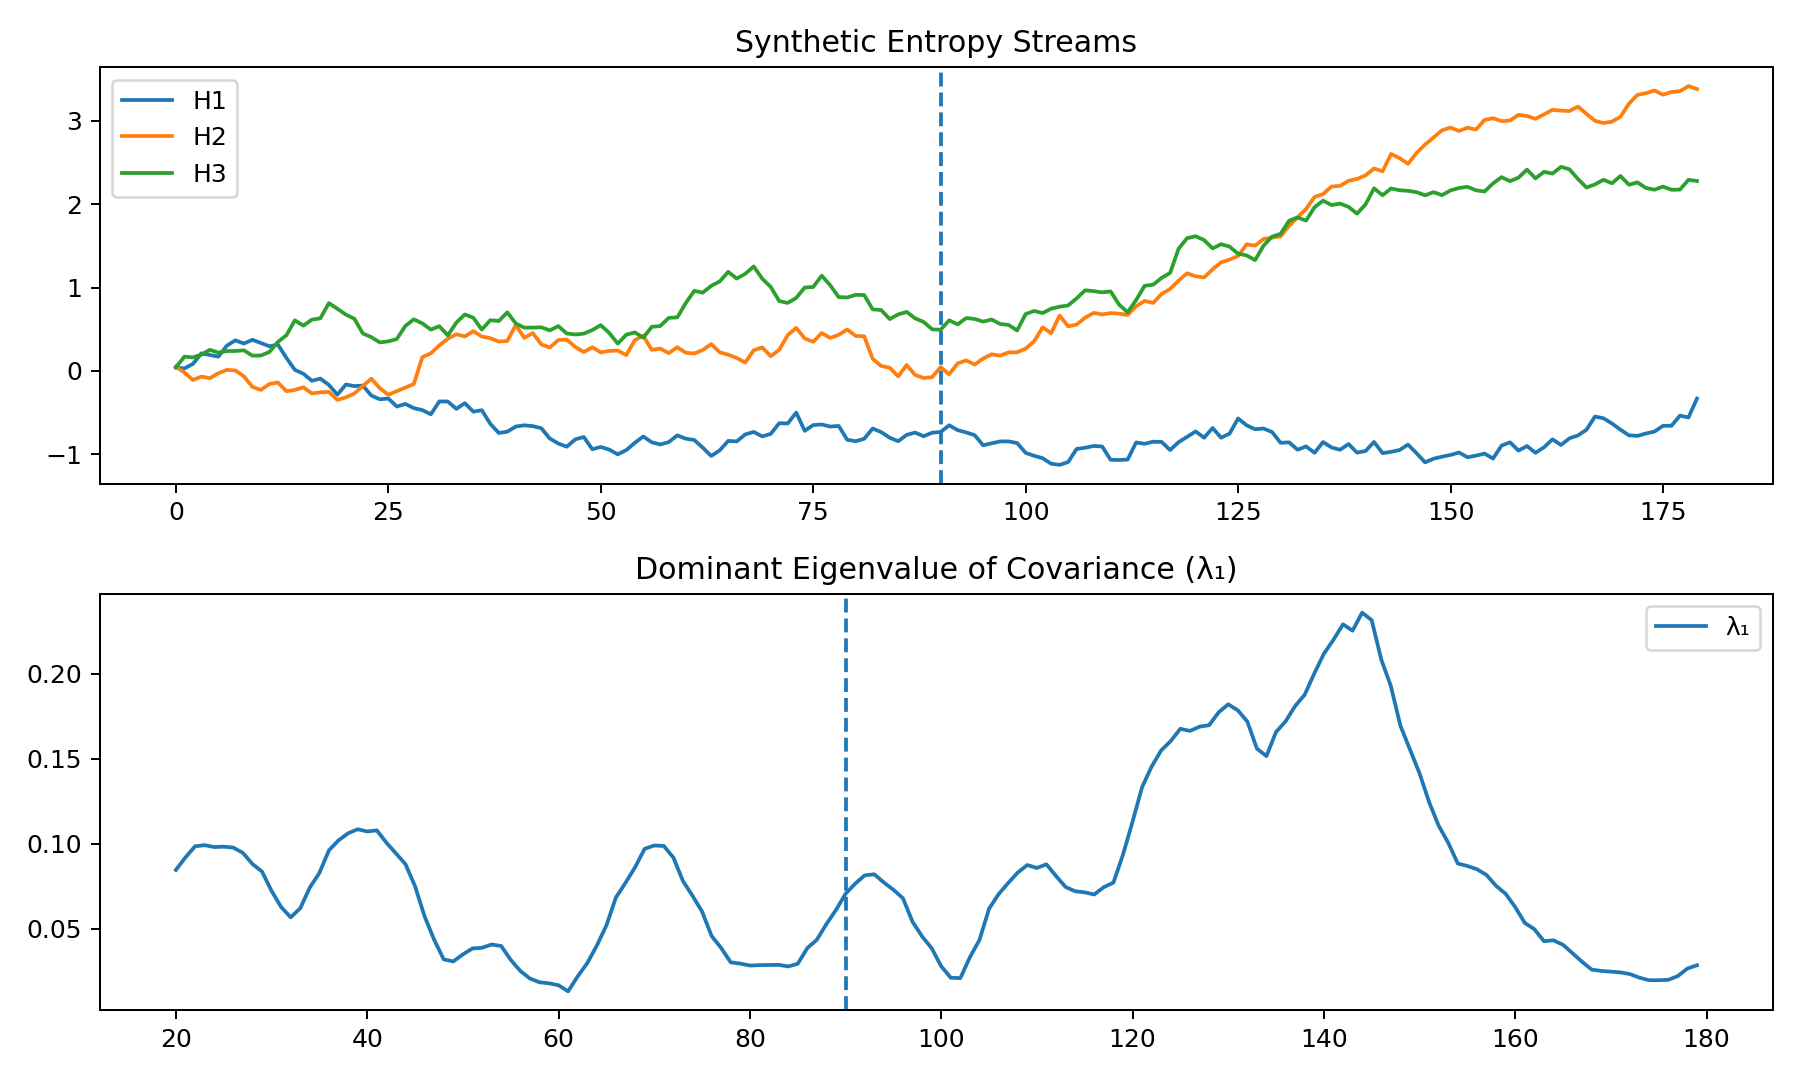
\includegraphics[width=0.8\textwidth]{toy_example_plot.png}
\caption{Toy example: entropy streams (top) and $\lambda_1$ of $\Sigma_H(t)$ (bottom). 
Spike at $t=50$ reveals systemic alignment.}
\end{figure}

\section{Implications}
\subsection{For SRE}
Eigenvalue spikes anticipate incidents by detecting alignment of uncertainties across metrics 
before threshold-based alerts fire.

\subsection{For Complex Systems}
Suggests a general mechanism for cascades: emergent failures are preceded by eigenmodes 
of entropy alignment.

\subsection{For AI Safety}
Provides a formalization of ``maternal instinct'' as sensitivity to entropy covariance. 
Systems can bias toward protective actions when shared uncertainty increases.

\section{Future Work}
\begin{itemize}
    \item Formalize within information geometry or statistical physics.
    \item Test across domains: ecosystems, economies, neuroscience.
    \item Embed entropy-covariance sensitivity in reinforcement learning agents.
\end{itemize}

\section{Conclusion}
Ted's Law of Karma compresses a universal idea: 
\emph{shared fate is visible in the covariance of entropies}.
This framing connects information theory, operations practice, and AI safety.

\bibliographystyle{plain}
\begin{thebibliography}{9}
\bibitem{Shannon1948} C. Shannon. ``A Mathematical Theory of Communication.'' Bell System Technical Journal, 1948.
\bibitem{Hinton2023} G. Hinton. ``The Need for Maternal Instinct in AI.'' (Talks, 2023).
\end{thebibliography}

\end{document}
